\documentclass[12pt]{article}
\usepackage{fullpage,url,amssymb,epsfig,color,xspace,amsmath}
\usepackage{graphicx}
\usepackage{slashbox}
\usepackage[]{algorithm2e}
\usepackage{pgfplots} % bar graphs
\usepackage{setspace}
\usepackage{tikz} %draw fancy pictures
\usepackage{verbatim}
\usetikzlibrary{calc,matrix}
\usepackage{caption}
\usepackage{amssymb}
\usepackage{amsmath}
\usepackage{amsthm}
\usepackage{graphicx}
\usepackage{mathtools}
\usepackage{enumitem}
\setlist{noitemsep} %set line separation of items to zero
\setlength\parindent{0pt} %no automatic indentation for new paragraph
\usetikzlibrary{arrows,shapes}
\usepackage{hyperref}
\usetikzlibrary{calc}
\setlength\parindent{0pt}
\usetikzlibrary{shapes.geometric}
\pgfplotsset{width=10cm,compat=1.8}
\newcommand{\pmtn}{\text{pmtn}}
\newcommand{\Note}{\paragraph{Note:}}
\newcommand{\Definition}{\paragraph{Definition}}
\newcommand{\Question}{\paragraph{Question}}
\newcommand{\Example}{\paragraph{Example}}
\newcommand{\Problem}{\paragraph{Problem}}
\newcommand{\Theorem}{\paragraph{Theorem}}
\newcommand{\tabfour}{\hspace*{100pt}}
\newcommand{\tabthree}{\hspace*{75pt}}
\newcommand{\tabtwo}{\hspace*{50pt}}
\newcommand{\tab}{\hspace*{25pt}}
\newcommand{\ra}{\rightarrow}
\newcommand{\Ra}{\Rightarrow}
\newcommand{\la}{\leftarrow}
\hypersetup{
	colorlinks=true, %set true if you want colored links
	linktoc=all,     %set to all if you want both sections and subsections linked
	linkcolor=blue,  %choose some color if you want links to stand out
}
\begin{document}
	
	\begin{center}
		\vspace*{3cm}	
		\textbf{\LARGE John Forbes Nash - First Edition}\\
		\vspace{5pt}
		\large Michael Ryan Blair, Xin Ye Liu, Mohammed Tahir Zaman, Brandon Yeh\\
		\vspace{5pt}
		CO480 - Spring 2015\\
	\end{center}
	
	\newpage
	
	\tableofcontents
	
	\newpage
	
	\singlespacing
	
	\section{Introduction to Game Theory \& Strategic Games}
	The creation of the field of Game Theory is largely attributed to John von Neumann and Oskar Morgenstern who fully introduced the concepts of cooperative games and 2-player zero-sum games in their paper \textit{Theory of Games and Economic Behaviour} (Nash’s Thesis). This exposition was published in 1944 and built on works published by the two authors dating back to 1928 (Theory of Games \& Economic Behaviour). This work provided a new approach to a number of problems in economics. \\
	
	Since this early work, the field of Game Theory has exploded. Game Theory has is used to study and explain phenomena not only in economics, but also in military tactics, biology, and in real-world corporate business decisions (e.g. Mergers \& Acquisitions, pricing decisions, supplier negotiations).
	
	\section{Strategic Games}
	
	We first define the class of games that Nash, and subsequently this paper will study. For the purposes of this paper, strategic games are games with N players, each of which has a finite number of pure strategies. This induces the following notation and definitions.
	
	\subsection{Definitions \& Notation}
	
	\Definition A strategic game with $N$ players has \textbf{player set} $\{1,...,n\}$ denoted by $N$\\
	
	Each player $i \in N$ has a finite number of pure strategies. The set of all of player i's strategies is denoted as $S_i$, and an individual pure strategy is denoted as $s_i$.\\
	
	A strategy profile denoted $S$ is a N-tuple, where each element $i$ is a pure strategy of player $i$.\\
	
	The collection of all strategy profiles $S$ is denoted as $\mathbb{S}$. We have then 
	\begin{equation*}
	\mathbb{S} = S_1 \times S_2 \times \cdots \times S_n
	\end{equation*} where $\times$ represents the Cartesian product of sets.\\
	
	We also define the following utility/payoff functions.
	
	\begin{equation*}
	\forall i, u_i : \mathbb{S} \Rightarrow \mathbb{R}
	\end{equation*}
	
	Each of the $u_i$ takes in a strategy profile and returns the utility value that the player receives under the strategy profile $S$. That is, if each player $i$ plays the strategy $s_i$ in S, the player $i$ will receive a payoff of $u_i(S)$
	
	\Note The specific payoff amount may have no meaning in a strategic game. The only claim is that a player prefers a higher payoff to a smaller payoff. We cannot, however, say that a player prefers a payoff of 2, twice as much as a payoff of 1.\\
	
	We also introduce the following substitution notation:\\
	
	Suppose $S = (s_1,...,s_n)$. Then the strategy profile $(S_{-i},s_i') = (s_i,...,s_{-1},s_i',s_{i+1},...,s_n)$. In words, $(S_{-1},s_i')$ is the strategy profile obtained from S when player $i$ changes their strategy from $s_i$ to $s_i'$\\
	
	\subsection{How are Strategic Games Played?}
	In strategic games each player moves simultaneously. That is, each player selects a strategy at the same time, and each player’s strategy selection is independent of the strategies chosen by the other players. Each player then receives payoff $u_i(S)$ based on the actions of each player.\\
	
	We make two key assumptions when playing strategic games:
	\begin{enumerate}
		\item Each player is a rational actor with the single goal of maximizing their own utility, meaning that a player will always choose the action that - given the other player’s strategies - will yield the highest payoff.\\
		
		\item We assume that players have played these games extensively in the past. It is assumed that this has led each player to form beliefs about how their opponents will play the game. This assumption is applied to each player, and it is assumed that all such beliefs are consistent.
	\end{enumerate}
	
	\subsection{Examples of Strategic Games}
	To illustrate strategic games, two-player games are often given in matrix form. The rows correspond to each of player 1’s moves, and the columns correspond to player 2’s moves. The elements of the matrix are ordered pairs (x, y) where x and y are the payoffs to player 1 and 2 respectively. 
	
	\newpage
	\paragraph{Prisoner's Dilemma\\}
	
Set-up: Two prisoners have been captured and are being interrogated about their involvement with a crime. Each prisoner has two options – remaining quiet (Q), or confessing (C). If both prisoners remain quiet, the police can only convict them of a minor charge. If both prisoners confess, the police will convict them of a major charge, but the sentence will be reduced because of their cooperation. If one prisoner confesses, they will go free and their accomplice will be convicted of the major offence. This situation can be modelled as the following strategic game:
	\begin{center}
	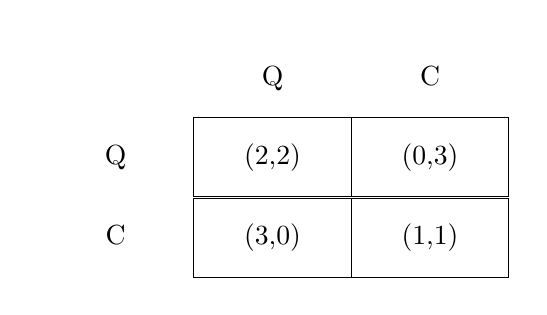
\begin{tikzpicture}[element/.style={minimum width=2cm,minimum height=1cm}]
	\matrix (m) [matrix of nodes,nodes={element},column sep=-\pgflinewidth, row sep=-\pgflinewidth,]{
		& Q  & C  \\
		Q & |[draw]|(2,2) & |[draw]|(0,3) \\
		C & |[draw]|(3,0) & |[draw]|(1,1) \\
	};
	
	\end{tikzpicture}
\end{center}

This results in the following instances of our definitions:
\begin{itemize}
	\item $\mathbb{S} = \{(Q,Q),(Q,C),(C,Q),(C,C)\}$
	\item $S_1 = S_2 = \{Q,C\}$
	\item $u_1((Q,Q)) = 1$
	\item $u_2((C,Q)) = 0$
\end{itemize}

\paragraph{Matching Pennies\\}

Set-up: Two players are each holding a penny. They each choose to show either Heads (H) or Tails (T). If both players select the same side, Player 2 pays player 1 \$1. If the sides do not match, then player 1 pays player 2 \$1.
This can be represented by the following matrix form:
\begin{center}
	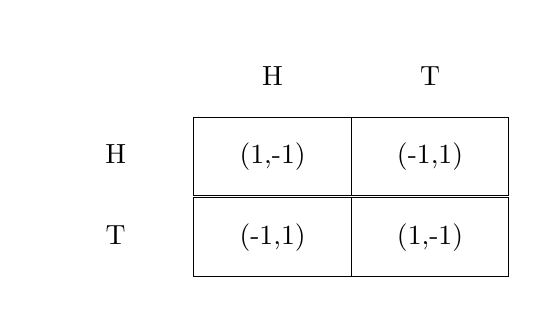
\begin{tikzpicture}[element/.style={minimum width=2cm,minimum height=1cm}]
	\matrix (m) [matrix of nodes,nodes={element},column sep=-\pgflinewidth, row sep=-\pgflinewidth,]{
		& H  & T  \\
		H & |[draw]|(1,-1) & |[draw]|(-1,1) \\
		T & |[draw]|(-1,1) & |[draw]|(1,-1) \\
	};
	
	\end{tikzpicture}
	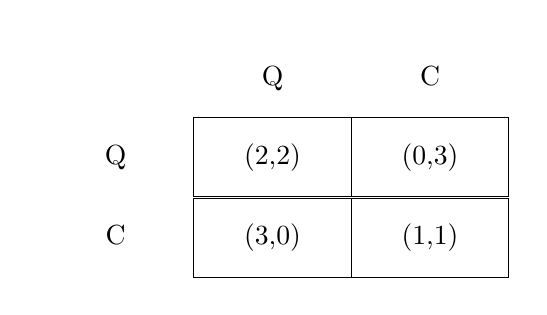
\begin{tikzpicture}[element/.style={minimum width=2cm,minimum height=1cm}]
		\matrix (m) [matrix of nodes,nodes={element},column sep=-\pgflinewidth, row sep=-\pgflinewidth,]{
			& Q  & C  \\
			Q & |[draw]|(2,2) & |[draw]|(0,3) \\
			C & |[draw]|(3,0) & |[draw]|(1,1) \\
		};
		
	\end{tikzpicture}
\end{center}

This results in the following instances of our definitions:
\begin{itemize}
	\item $\mathbb{S} = \{(H,H),(H,T),(T,H),(T,T)\}$
	\item $S_1 = S_2 = \{H,T\}$
	\item $u_1((H,H)) = 1$
	\item $u_2((H,H)) = -1$
\end{itemize}


\end{document}